
\chapter{Μαθηματικό και θεωρητικό υπόβαθρο}
\numberwithin{equation}{section}

\section{Διανύσματα βάσης}
\par
Έστω ότι έχουμε ένα σύνολο δειγμάτων εισόδου με αντίστοιχο διάνυσμα \textlatin{\textbf{x}} διάστασης $N\times1$,
\newline\hspace*{\fill}
$\mathbf{x}^{T} = \begin{bmatrix}
        x(0),\ldots,x(N-1)
        \end{bmatrix}$
\hspace*{\fill}\newline
\newline
Έστω επίσης ορθοκανονικό μητρώο Α, τάξης $Ν\timesΝ$. Τότε ορίζουμε το μετασχηματισμένο διάνυσμα \textlatin{\textbf{y}} του \textlatin{\textbf{x}} ως 
\newline\hspace*{\fill}
\begin{equation}
        \mathbf{y} = \mathbf{A}^{H}\mathbf{x} \equiv \begin{bmatrix}
       \mathbf{a}_{0}^{H} \\
       \vdots \\
       \mathbf{a}_{N-1}^{H} \\
     \end{bmatrix} \mathbf{x}
\end{equation}
\hspace*{\fill}\newline
\newline
Το H δηλώνει τον \textlatin{Hermitian} τελεστή, δηλαδή τον μιγαδικό συζυγή του ανάστροφου. Από τον ορισμό των ορθοκανονικών μητρώων έχουμε   
\newline\hspace*{\fill}
\begin{equation}
        \mathbf{x} = \mathbf{Ay} = \sum_{i=0}^{N-1} y(i)\mathbf{a}_{i}
\end{equation}
\hspace*{\fill}\newline
\newline
Οι στήλες του \textbf{\textlatin{A}}, $\mathbf{a}_{i}=0,1,\ldots,N-1$ καλούνται \textit{διανύσματα βάσης} του μετασχηματισμού. Τα στοιχεία $y(i)$ του $\mathbf{y}$ είναι οι προβολές του διανύσματος $\mathbf{x}$ σε αυτά τα διανύσματα βάσης. Λαμβάνοντας υπόψιν την ιδιότητα της ορθοκανονικότητας μπορούμε να επαληθεύσουμε την παραπάνω διατύπωση υπολογίζοντας το εσωτερικό γινόμενο του $\mathbf{x}$ με το $\mathbf{a}_{j}$. Έχουμε:
\newline\hspace*{\fill}
\begin{equation}
        \langle\mathbf{a}_{j},\mathbf{x}\rangle \equiv \mathbf{a}_{j}^{H}\mathbf{x} = \sum_{i=0}^{N-1} y(i)\langle\mathbf{a}_{j},\mathbf{a}_{i}\rangle = \sum_{i=0}^{N-1} y(i)\delta_{ij} = y(j)
\end{equation}
\hspace*{\fill}

\subsection{Διάνυσμα εικόνας}
\par
Αν πάρουμε για παράδειγμα μια εικόνα, το σύνολο των δειγμάτων εισόδου είναι μια δισδιάστατη ακολουθία $X(i,j), i,j=0,1,\ldots,N-1$, η οποία ορίζει ένα μητρώο $Χ$, τάξεως $Ν\timesΝ$. Σε αυτή την περίπτωση  μπορούμε να μετατρέψουμε την είσοδο αυτή σε ένα διάνυσμα  $\mathbf{x}$ διάστασης $N^{2}$ διατάσσοντας για παράδειγμα τις γραμμές του μητρώου την μία μετά την άλλη έχοντας τελικά \\
\newline\hspace*{\fill}
\begin{equation}
        \mathbf{x}^{T} = \begin{bmatrix}
        X(0,0),\ldots,X(0,N-1),\ldots,X(N-1,0),\ldots,X(N-1,N-1)
        \end{bmatrix}
\end{equation}
\hspace*{\fill}\newline
\newline
Με αυτό τον μετασχηματισμό όμως ο αριθμός των πράξεων που απαιτούνται για τον πολλαπλασιασμό ενός τετραγωνικού μητρώου τάξεως $Ν\timesΝ$ με ένα διάνυσμα $\mathbf{x}$ διαστάσεων $N^{2}\times1$, είναι της τάξης $\mathcal{O}(Ν^{4})$ μέγεθος απαγορευτικό για τις περισσότερες ρεαλιστικές εφαρμογές.

\subsection{Ορθοκανονικά ιδιοδιανύσματα}
\par
Το παραπάνω εμπόδιο μπορεί να ξεπεραστεί αν μετασχηματίσουμε το μητρώο $Χ$ μέσω ενός συνόλου \textit{μητρώων βάσης}. Έστω λοιπόν $U$ και $V$ ορθοκανονικά μητρώα διάστασης $Ν\timesΝ$. Ορίζουμε τότε το μετασχηματισμένο μητρώο $Y$ του $X$ ως
\newline\hspace*{\fill}
\begin{equation}
        Y=U^{H} XV
\end{equation}
\hspace*{\fill}\newline
ή
\newline\hspace*{\fill}
\begin{equation}
        X=UYV^{H}
\end{equation}
\hspace*{\fill}\newline
\newline
Μέσω αυτού του μετασχηματισμού ο αριθμός των πράξεων μειώνεται σε $\mathcal{O}(N^{3})$. Πιο αναλυτικά η παραπάνω εξίσωση θα μπορούσε να γραφεί ως
\newline\hspace*{\fill}
\begin{equation}
        Χ = \sum_{i=0}^{N-1} \sum_{j=0}^{N-1} Y(i,j)\mathbf{u}_{i}\mathbf{v}_{j}^{H}
\end{equation}
\hspace*{\fill}\newline
\newline
όπου $\mathbf{u}_{i}$ είναι τα διανύσματα στήλης του \textlatin{U} και $\mathbf{v}_{j}$ τα διανύσματα στήλης του \textlatin{V}. Η παραπάνω εξίσωση είναι ένα ανάπτυγμα του μητρώου \textlatin{X} ως προς τις $Ν\times2$ εικόνες βάσης. Τέλος κάθε ένα από τα γινόμενα $\mathbf{u}_{i}\mathbf{v}_{j}$ είναι ένα μητρώο $Ν\timesΝ$ \\
\newline\hspace*{\fill}
\begin{equation}
        \mathbf{u}_{i}\mathbf{v}_{j}=\begin{bmatrix}
        u_{i0}v_{j0}^{*}	 &	\ldots  &  u_{i0}v_{jN-1}^{*} 	\\
        \vdots				 &  	\vdots  &  \vdots \\
        u_{iN-1}v_{j0}^{*} &    	\ldots  &  u_{iN-1}v_{jN-1}^{*} \\
        \end{bmatrix}
\end{equation}
\hspace*{\fill}\newline
\newline
Στην περίπτωση κατα την οποία το \textlatin{Y} είναι διαγώνιο τότε έχουμε \\
\newline\hspace*{\fill}
\begin{equation}
        Χ = \sum_{i=0}^{N-1} Y(i,i)\mathbf{u}_{i}\mathbf{v}_{i}^{H}
\end{equation}
\hspace*{\fill}\newline
\newline
με αποτέλεσμα το πλήθος των μητρώων-εικόνων βάσης να μειώνεται σε Ν. Τέλος έπειτα από μερικές πράξεις και τροποποιήσεις μπορούμε να ορίσουμε κάθε στοιχείο $(i,j)$ του μετασχηματισμένου μητρώου ως τον πολλαπλασιασμό κάθε στοιχείου του Χ με τον συζυγή του αντίστοιχου στοιχείου του $Α_{ij}$ και αθροίζοντας όλα τα γινόμενα. Δηλαδή
\newline\hspace*{\fill}
\begin{equation}
        \langle A,B \rangle = \sum_{m=0}^{N-1} \sum_{n=0}^{N-1} A(m,n)^{*}B(m,n)
\end{equation}
\hspace*{\fill}\newline
και τελικά
\newline\hspace*{\fill}
\begin{equation}
        Y(i,j) = \langle A_{i,j},X \rangle
\end{equation}
\hspace*{\fill}\newline

\section{Ο μετασχηματισμός \textlatin{Karhunen-Loeve} - \textlatin{PCA}}
\par
Ο μετασχηματισμός \textlatin{Karhunen-Loeve}\textlatin{\cite{pca}} αξιοποιεί την στατιστική πληροφορία που περιγράφει τα δεδομένα και ο υπολογισμός του μητρώου γίνεται χωρίς επίβλεψη. Ας υποθέσουμε και πάλι ένα διάνυσμα $\mathbf{x}$ το οποίο αποτελείται από τα δείγματα μια εικόνας τα οποία έχουν διαταχθεί λεξικογραφικά όπως περιγράφτηκε παραπάνω. Πρέπει να επισημανθεί στο σημείο αυτό η επιθυμητή ιδιότητα των εξαχθέντων χαρακτηριστικών να είναι αμοιβαίως ασυσχέτιστα και αυτό για την αποφυγή πλεονάζουσας πληροφορίας. Η πιο συνηθισμένη συνθήκη για την γέννηση τέτοιου είδους χαρακτηριστικών είναι η μέση τιμή των δεδομένων να έχει μηδενική τιμή. Δηλαδή θέλουμε την ιδιότητα
\newline\hspace*{\fill}
\begin{equation}
        Ε[y(i)y(j)]=0,i \neq j
\end{equation}
\hspace*{\fill}\newline
Έστω 
\newline\hspace*{\fill}
\begin{equation}
        \mathbf{y} = A^{T}\mathbf{x}
\end{equation}
\hspace*{\fill}\newline
Εφόσον έχουμε υποθέσει ότι $Ε[x]=0$ αμέσως βλέπουμε ότι $Ε[y]=0$ και 
\newline\hspace*{\fill}
\begin{equation}
        R_{y}=E[\mathbf{y}\mathbf{y}^{T}]=E[A^{T} \mathbf{x}\mathbf{x}^{T} A]=A^{T}R_{x}A
\end{equation}
\hspace*{\fill}\newline
Πρακτικά το $R_{x}$ αντιπροσωπεύει μια μέση τιμή πάνω στο δοθέν σύνολο διανυσμάτων εκπαίδευσης. Επίσης είναι συμμετρικό μητρώο και επομένως τα ιδιοδιανύσματά του είναι αμοιβαίως ορθογώνια. Άρα έστω ότι επιλέγεται ένα μητρώο Α με στήλες τα ορθοκανονικά ιδιοδιανύσματα $\mathbf{a}_{i},i=0,1,\ldots,N-1$ του $R_{x}$  τότε το $R_{y}$ είναι διαγώνιο.
\newline\hspace*{\fill}
\begin{equation}
        R_{y}=A^{T}R_{x}A=\Lambda
\end{equation}
\hspace*{\fill}\newline
Το $\Lambda$ είναι διαγώνιο μητρώο με διαγώνια στοιχεία τις αντίστοιχες ιδιοτιμές $\lambda_{i},i=0,1,\ldots,N-1$ του $R_{x}$. Αποτέλεσμα της παραπάνω διαδικασίας είναι ένας μετασχηματισμός, ο μετασχηματισμός \textlatin{Karhunen-Loeve}, ο οποίος επιτυγχάνει τον αρχικό μας στόχο, δηλαδή την δημιουργία χαρακτηριστικών τα οποία είναι στατιστικώς ανεξάρτητα.

\subsection{Προσέγγιση μέσου τετραγωνικού σφάλματος - \textlatin{MSE}}
\par
Σε αυτή την υποενότητα θα αναλυθεί η διαδικασία με την οποία μπορούμε να οδηγηθούμε στην επιλογή κάποιων, έστω \textlatin{m} το πλήθος, κυρίαρχων χαρακτηριστικών μέσω της προσέγγισης μέσου τετραγωνικού σφάλματος. Ας πάρουμε ξανά τις εξισώσεις  (2.1.1) και (2.1.2) τότε έχουμε
\newline\hspace*{\fill}
\begin{equation}
        \mathbf{x} = \sum_{i=0}^{N-1} y(i)\mathbf{a}_{i} \quad \text{και} \quad y(i)=\mathbf{a}_{i}^{T}\mathbf{x}
\end{equation}
\hspace*{\fill}\newline
Ορίζουμε λοιπόν τώρα ένα νέο διάνυσμα στον \textlatin{m}-διάστατο υποχώρο
\newline\hspace*{\fill}
\begin{equation}
        \mathbf{\widehat{x}} = \sum_{i=0}^{m-1} y(i)\mathbf{a}_{i}
\end{equation}
\hspace*{\fill}\newline
στο οποίο προφανώς εμπλέκονται μόνο \textlatin{m} από τα διανύσματα βάσης. Με τον παραπάνω τρόπο δηλαδή ορίζεται η προβολή του $\mathbf{x}$ στον υποχώρο που ορίζουν τα ορθοκανονικά διανύσματα \textlatin{m} τα οποία εμπλέκονται στην παραπάνω άθροιση. 
\par
Σκοπός μας λοιπόν στο σημείο αυτό είναι να προσεγγίσουμε με όσο το δυνατόν μικρότερο σφάλμα το διάνυσμα $\mathbf{x}$. Η προσέγγισή μας είναι το διάνυσμα $\mathbf{\widehat{x}}$ και θα προκύψει χρησιμοποιώντας την εξίσωση ελαχιστοποίησης μέσου τετραγωνικού σφάλματος. Έχουμε λοιπόν την εξίσωση 
\newline\hspace*{\fill}
\begin{equation}
        Ε[{\Vert \mathbf{x}-\mathbf{\widehat{x}} \Vert}^{2}] = E 			\begin{bmatrix}
	{\Vert \sum_{i=m}^{N-1} y(i)\mathbf{a}_{i} \Vert}^{2}        
        \end{bmatrix}
\end{equation}
\hspace*{\fill}\newline
Από την παραπάνω εξίσωση στόχος μας τώρα είναι να επιλέξουμε τα ιδιοδιανύσματα τα οποία οδηγούν στο ελάχιστο μέσο τετραγωνικό σφάλμα. Λαμβάνοντας υπόψιν την ορθοκανονικότητα των ιδιοδιανυσμάτων και την παραπάνω εξίσωση καταλήγουμε ότι
\newline\hspace*{\fill}
\begin{equation}
 	Ε   \begin{bmatrix}
	{\Vert \sum_{i=m}^{N-1} y(i)\mathbf{a}_{i} \Vert}^{2}        
        \end{bmatrix}
    = Ε \begin{bmatrix}
	\sum_{i}\sum_{j} (y(i)\mathbf{a}_{i}^{T})(y(j)\mathbf{a}_{j})        
        \end{bmatrix} = 
\end{equation}
\hspace*{\fill}
\newline\hspace*{\fill}
\begin{equation}
    = \sum_{i=m}^{N-1} E[y^{2}(i)]
    = \sum_{i=m}^{N-1} \mathbf{a}_{i}^{T} E[\mathbf{x}\mathbf{x}^{T}]\mathbf{a}_{i}
\end{equation}
\hspace*{\fill}\newline
και λαμβάνοντας υπόψιν τον ορισμό των ιδιοδιανυσμάτων προκύπτει τελικά ότι
\newline\hspace*{\fill}
\begin{equation}
         Ε[{\Vert \mathbf{x}-\mathbf{\widehat{x}} \Vert}^{2}] = \sum_{i=m}^{N-1} \mathbf{a}_{i}^{Τ}\lambda_{i}\mathbf{a}_{i} = 
         \sum_{i=m}^{N-1} \lambda_{i} 
\end{equation}
\hspace*{\fill}\newline
Αν επομένως στην παραπάνω εξίσωση επιλέξουμε τα ιδιοδιανύσματα που αντιστοιχούν στις \textlatin{m} ιδιοτιμές του μητρώου συσχέτισης τότε το σφάλμα της εξίσωσης ελαχιστοποιείται και μάλιστα ισούται με το άθροισμα των \textlatin{N-m} μικρότερων ιδιοτιμών. Επιπλέον έχει αποδειχθεί ότι αυτό είναι το ελάχιστο μέσο τετραγωνικό σφάλμα σε σύγκριση με οποιαδήποτε άλλη προσέγγιση του \textlatin{\textbf{x}} από ένα \textlatin{m}-διάστατο διάνυσμα. Για τον λόγο αυτό ο μετασχηματισμός \textlatin{Karhunen-Loeve} είναι επίσης γνωστός ως \textit{Ανάλυση κυρίων συνιστωσών} \textlatin{(Principal component analysis-PCA)}.

\subsection{Συνολική Διασπορά}
\par
Έστω \textlatin{\textbf{y}} το μετασχηματισμένο κατά \textlatin{\textbf{KL}} διάνυσμα του \textlatin{\textbf{x}} και $E[x]=0$. Τότε από τον αντίστοιχο ορισμό της διασποράς έχουμε ότι $\sigma^{2}_{y(i)} \equiv E[y^{2}(i)]=\lambda_{i}$. Δηλαδή έχουμε ότι οι διασπορές του μητρώου συσχέτισης εισόδου είναι ίσες με τις διασπορές των μετασχηματισμένων χαρακτηριστικών. Επομένως επιλέγοντας εκείνα τα χαρακτηριστικά $ y(i)=\mathbf{a}_{i}^{T}\mathbf{x} $ που αντιστοιχούν στις \textlatin{m} μεγαλύτερες ιδιοτιμές οδηγούμαστε σε μεγιστοποίηση της αθροιστικής διασποράς $ \sum_{i} \lambda_{i} $. Συμπεραίνουμε λοιπόν ότι με αυτή την μεθοδολογία που ακολουθήσαμε, τα \textlatin{m} χαρακτηριστικά που έχουν επιλεχθεί διατηρούν το μεγαλύτερο μέρος από την συνολική διασπορά που σχετίζεται με τις αρχικές τυχαίες μεταβλητές $x(i)$.

\subsection{Μείωση της διάστασης μέσω \textlatin{PCA}}
\par
Απο την παραπάνω ανάλυση είναι φανερό ότι η μέθοδος \textlatin{PCA}\textlatin{\cite{pca}} επιτυγχάνει τον \textit{γραμμικό μετασχηματισμό} ενός χώρου υψηλής διάστασης σε έναν χαμηλής διάστασης του οποίου μάλιστα τα στοιχεία είναι στατιστικώς ασυσχέτιστα. Έχοντας υποθέσει ότι $E[x]=0$ και επίσης ότι οι \textlatin{N-m} μικρότερες ιδιοτιμές του μητρώου συσχέτισης είναι μηδέν τότε από την εξίσωση (2.2.10) συνεπάγεται ότι $\mathbf{x} = \mathbf{\widehat{x}}$. Δηλαδή έχουμε ότι το διάνυσμα $\mathbf{x}$ του αρχικού χώρου διάστασης \textlatin{N} βρίσκεται σε έναν \textlatin{m}-διάστατο υποχώρο του αρχικού και μάλιστα μπορούμε να το προσδιορίσουμε μέσω του διανύσματος $\mathbf{\widehat{x}}$ με πολύ καλή προσέγγιση. Το γεγονός αυτό εισάγει την έννοια της \textit{εγγενούς διάστασης} (\textlatin{intrinsic dimensionality}). Τέλος στην περίπτωση της εγγενούς διάστασης μπορούμε να πούμε ό,τι το \textlatin{X} μπορεί να περιγραφεί από \textlatin{m} ελεύθερες παραμέτρους.

\section{Μετρική πολυδιάστατης κλιμάκωσης (\textlatin{Metric multidimensional scaling - MDS})}
\par
Ένας ακόμα πολύ διαδεδομένος αλγόριθμος μείωσης διάστασης είναι ο αλγόριθμος \textit{Μετρική πολυδιάστατης κλιμάκωσης} (\textlatin{Metric multidimensional scaling - MDS})\textlatin{\cite{mds}}. Ο αλγόριθμος αυτός δοθέντος ενός συνόλου $Χ\subset\Re^{N}$, έχει ως στόχο να γίνει προβολή σε χώρο χαμηλότερης διάστασης, $Y\subset\Re^{m}$, έτσι ώστε τα εσωτερικά γινόμενα να διατηρηθούν κατά βέλτιστο τρόπο. Πρέπει δηλαδή να γίνει η ελαχιστοποίηση της εξίσωσης
\newline\hspace*{\fill}
\begin{equation}
        E = \sum_{i} \sum_{j} (\mathbf{x}_{i}^{T}\mathbf{x}_{j}-\mathbf{y}_{i}^{T}\mathbf{y}_{j})^{2}
\end{equation}
\hspace*{\fill}\newline
όπου $\mathbf{y}_{i}$ είναι η εικόνα του $\mathbf{x}_{i}$ και το άθροισμα υπολογίζεται ως προς όλα τα σημεία εκπαίδευσης του $X$. Το πρόβλημα δηλαδή, και σε αυτή την περίπτωση είναι όμοιο με αυτό της μεθόδου \textlatin{PCA}, και μπορεί να αποδειχθεί ότι η λύση δίνεται από την ανάλυση σε ιδιοτιμές-ιδιοδιανύσματα του μητρώου \textlatin{Gram}, τα στοιχεία του οποίου ορίζονται ως 
\newline\hspace*{\fill}
\begin{equation}
        K(i,j) = \mathbf{x}_{i}^{T}\mathbf{x}_{j}
\end{equation}
\hspace*{\fill}\newline
\par
Ένας εναλλακτικός τρόπος επίλυσης του προβλήματος είναι η απαίτηση να διατηρηθούν, κατά βέλτιστο τρόπο, οι Ευκλείδιες αποστάσεις αντί των εσωτερικών γινομένων. Μπορούμε έτσι, να δημιουργήσουμε ένα μητρώο \textlatin{Gram} συμβατό με τις τετραγωνικές Ευκλείδιες αποστάσεις, το οποίο μας οδηγεί στην ίδια λύση όπως και στην προηγούμενη περίπτωση. Προκύπτει μάλιστα, ότι οι λύσεις που προκύπτουν απο τις μεθόδους \textlatin{PCA}\textlatin{\cite{pca}} και \textlatin{MDS}\textlatin{\cite{mds}} είναι ισοδύναμες.
\par
Μια σύντομη απόδειξη της παραπάνω διατύπωσης είναι η εξής. Η μέθοδος \textlatin{PCA} εκτελεί την ανάλυση ιδιοτιμών του μητρώου συσχέτισης $R_{x}$, το οποίο προσεγγίζεται από τη σχέση
\newline\hspace*{\fill}
\begin{equation}
        R_{x} = E[\mathbf{x}\mathbf{x}^{T}] \approx \dfrac{1}{n} \sum_{k=1}^{n} \mathbf{x}_{k}\mathbf{x}_{k}^{T} = \dfrac{1}{n} X^{T}X
\end{equation}
\hspace*{\fill}\newline
όπου 
\newline\hspace*{\fill}
\begin{equation}
        X^{Τ} = [\mathbf{x}_{1},\mathbf{x}_{2},\ldots,\mathbf{x}_{n},]
\end{equation}
\hspace*{\fill}\newline
Απο την άλλη το μητρώο \textlatin{Gram} μπορεί επίσης να γραφεί ως 
\newline\hspace*{\fill}
\begin{equation}
        K = XX^{T}
\end{equation}
\hspace*{\fill}\newline
Τέλος αποδεικνύεται ότι τα δύο μητρώα $X^{T}X$ και $XX^{T}$ είναι ίδιου βαθμού και έχουν τις ίδιες ιδιοτιμές με ιδιοδιανύσματα τα οποία ναι μεν είναι διαφορετικά μεταξύ τους αλλά παρόλα αυτά σχετίζονται.

\section{Ανάλυση στην βάση των ιδιαζουσών τιμών (\textlatin{Singular Value Decomposition - SVD})}
\par
Η ανάλυση ενός μητρώου με βάση τις ιδιάζουσες τιμές είναι μια από τις πιο κομψές και ισχυρές μεθόδους γραμμικής άλγεβρας η οποία έχει χρησιμοποιηθεί εκτενώς για την μείωση του βαθμού και της διάστασης σε προβλήματα αναγνώρισης προτύπων και σε εφαρμογές ανάκτησης πληροφορίας.
\par
Δοθέντος ενός μητρώου Χ, τάξης $l \times n$, βαθμού \textlatin{r} με $r \leq \min \lbrace \textlatin{l,n} \rbrace $ υπάρχουν ορθοκανονικά μητρώα \textlatin{U} και \textlatin{V}, τάξης $l \times l$ και $n \times n$ αντίστοιχα ώστε
\newline\hspace*{\fill}
\begin{equation}
	X = U\begin{bmatrix}
	\Lambda^{\frac{1}{2}} & \mathcal{O} \\
	\mathcal{O} & 0
	\end{bmatrix} V^{H} \quad \text{ή} \quad
	Y = \begin{bmatrix}
	\Lambda^{\frac{1}{2}} & \mathcal{O} \\
	\mathcal{O} & 0
	\end{bmatrix} = U^{H}XV 
\end{equation}
\hspace*{\fill}\newline
όπου $ \Lambda^{\frac{1}{2}} $ είναι το $r \times r$ διαγώνιο μητρώο με στοιχεία $ \sqrt{\lambda_{i}} $ με $ \lambda_{i} $ οι μη μηδενικές ιδιοτιμές που σχετίζονται με το μητρώο $X^{H}X$. Με $ \mathcal{O} $ συμβολίζουμε το μητρώο μηδενικών τιμών. Από τα παραπάνω γίνεται φανερό ότι υπάρχουν μητρώα \textlatin{U} και \textlatin{V} που μετασχηματίζουν το \textlatin{X} στην διαγώνια δομή του \textlatin{Y}. Αν $ \mathbf{u}_{i}$,$\mathbf{v}_{i} $ είναι τα διανύσματα στήλης των μητρώων \textlatin{U} και \textlatin{V} αντίστοιχα τότε η παραπάνω εξίσωση μπορεί να γραφεί στην μορφή
\newline\hspace*{\fill}
\begin{equation}
         X = [u_{0},u_{1},\ldots,u_{r-1},] \begin{bmatrix}
\sqrt{\lambda_{0}} &&&& \\
&\sqrt{\lambda_{1}} &&& \\
&& \raise 4pt \hbox {.}
  \mkern 6mu
  \raise 1pt \hbox {.}
  \mkern 6mu
  \raise -2pt \hbox {.} \\
&&& \sqrt{\lambda_{r-1}} \\
\end{bmatrix}
\begin{bmatrix}
	\mathbf{v}_{0}^{H} \\
	\mathbf{v}_{1}^{H} \\
	\vdots \\
	\mathbf{v}_{r-1}^{H} \\
\end{bmatrix}
\end{equation}
\hspace*{\fill}\newline
ή
\newline\hspace*{\fill}
\begin{equation}
	X = \sum_{i=0}^{r-1} \sqrt{\lambda_{i}} \mathbf{u}_{i}\mathbf{v}_{i}^{H} = U_{r}\Lambda^{\frac{1}{2}}V_{r}^{H}
\end{equation}
\hspace*{\fill}\newline
όπου $U_{r}$ δηλώνει το $l \times r$ μητρώο που αποτελείται απο τις \textlatin{r} πρώτες στήλες του \textlatin{U} και $V_{r}$ το $r \times n$ μητρώο που σχηματίζεται χρησιμοποιώντας τις πρώτες \textlatin{r} στήλες του \textlatin{V}. Επίσης $ \mathbf{u}_{i} $,$ \mathbf{v}_{i} $ είναι τα ιδιοδιανύσματα που αντιστοιχούν στις μη μηδενικές ιδιοτιμές των μητρώων $XX^{H}$ και $X^{H}X$ αντίστοιχα. Οι ιδιοτιμές $ \lambda_{i} $ είναι γνωστές ως \textit{ιδιάζουσες τιμές} \textlatin{(singular values)} του $X$ και το ανάπτυγμα της παραπάνω εξίσωσης ως \textit{ανάλυση με βάση τις ιδιάζουσες τιμές} \textlatin{(singular value decomposition - SVD)\textlatin{\cite{svd}\cite{13}}} του $X$.
\subsection{Μείωση της διάστασης μέσω \textlatin{SVD}}
\par
Η μέθοδος \textlatin{SVD}\textlatin{\cite{svd}\cite{13}} έχει χρησιμοποιηθεί εκτενώς για την μείωση της διάστασης του χώρου χαρακτηριστικών σε ένα μεγάλο εύρος εφαρμογών αναγνώρισης προτύπων. Έστω οτι έχουμε την προσέγγιση χαμηλού βαθμού \textlatin{(low rank approximation)} $ \hat{X} $ του \textlatin{X}. Αποδεικνύεται μέσω ελαχιστοποίησης του μέσου τετραγωνικού σφάλματος ότι αν η παραπάνω προσέγγιση σχηματίζεται απο την άθροιση των \textlatin{k} μεγαλύτερων ιδιοτιμών τότε το μέσο τετραγωνικό σφάλμα της προσέγγισης είναι το ελάχιστο. Μπορούμε να καταλήξουμε στο συμπέρασμα ότι η μέθοδος \textlatin{SVD}\textlatin{\cite{svd}\cite{13}} οδηγεί στο ελάχιστο τετραγωνικό σφάλμα και επομένως το $ \hat{X} $ είναι η καλύτερη \textit{προσέγγιση βαθμού \textlatin{k}} του \textlatin{X}. Η προσέγγιση αυτή δίνεται από τον τύπο \\
\newline\hspace*{\fill}
$ X \simeq \hat{X} = \sum_{i=0}^{k-1} \sqrt{\lambda_{i}} \mathbf{u}_{i}\mathbf{v}_{i}^{H},\quad k \leq r $
\hspace*{\fill}\newline
\newline\hspace*{\fill}
\begin{equation}
	= [\mathbf{u}_{0},\mathbf{u}_{1},\ldots,\mathbf{u}_{k-1}]
	\begin{bmatrix}
	\sqrt{\lambda_{0}}\mathbf{v}_{0}^{H} \\
	\sqrt{\lambda_{1}}\mathbf{v}_{1}^{H} \\
	\vdots \\ 
	\sqrt{\lambda_{k-1}}\mathbf{v}_{k-1}^{H}
	\end{bmatrix} 
	= U_{k}[\mathbf{a}_{0},\mathbf{a}_{1},\ldots,\mathbf{a}_{n-1},]
\end{equation}
\hspace*{\fill}\newline
όπου ο μητρώο $U_{k}$ αποτελείται από τις \textlatin{k} πρώτες στήλες του $U$ και τα \textlatin{k}-διάστατα διανύσματα $\mathbf{a}_{i},i=0,1,\ldots,n-1$ είναι τα διανύσματα στήλες της $k \times n$ μήτρας του γινομένου $ \Lambda^{\frac{1}{2}}V_{k}^{H}$. Το μητρώο $V_{k}^{H}$ αποτελείται από τις $k$ πρώτες γραμμές του $V^{H}$ και $ \Lambda^{\frac{1}{2}} $ είναι διαγώνιο μητρώο με στοιχεία τις τετραγωνικές ρίζες των αντίστοιχων $k$ ιδιαζουσών τιμών.
\par
Στο παρακάτω σχήμα παρουσιάζεται γραφικά ώστε να γίνει καλύτερα κατανοητή η παραπάνω διαδικασία. \\
\vspace*{6cm}
\begin{figure}[h]
\centering
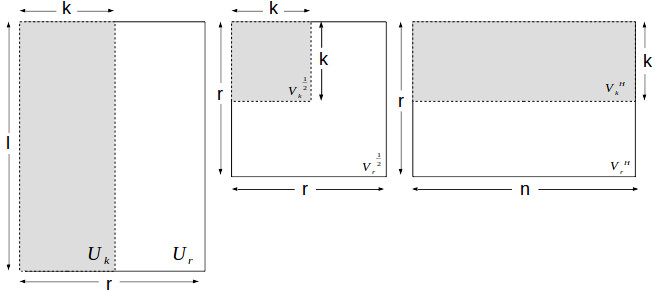
\includegraphics[scale=0.7]{figs/1.jpg}
\newline
\caption{Μείωση της διάστασης με \textlatin{SVD}} 
\end{figure}
\par
\vspace*{2cm}
Απο την παραπάνω ανάλυση καταλήγουμε στο συμπέρασμα ότι το \textlatin{l}-διάστατο διάνυσμα $ \mathbf{x}_{i} $ προσεγγίζεται απο το \textlatin{k}-διάστατο διάνυσμα $ \mathbf{a}_{i} $ που βρίσκεται στον υποχώρο που ορίζουν τα $ \mathbf{u}_{i},i=0,1,\ldots,k-1$ (το $ \mathbf{a}_{i}$ είναι στην ουσία η προβολή του $ \mathbf{x}_{i} $ στον υποχώρο αυτόν). Επίσης, λόγω της ορθοκανονικότητας των στηλών $ \mathbf{u}_{i},i=0,1,\ldots,k-1 $ του $ U_{k} $ βλέπουμε ότι
\newline\hspace*{\fill}
\begin{equation}
	\Vert \mathbf{x}_{i}-\mathbf{x}_{j} \Vert \simeq \Vert U_{k}(\mathbf{a}_{i}-\mathbf{a}_{j}) \Vert = \Vert \sum_{m=0}^{k-1} \mathbf{u}_{m} (a_{i}(m)-a_{j}(m)) \Vert = \Vert \mathbf{a}_{i}-\mathbf{a}_{j}\Vert, \quad i,j=0,1,\ldots,n-1
\end{equation}
\hspace*{\fill}\newline
Αντιλαμβανόμαστε λοιπόν ότι χρησιμοποιώντας την προηγούμενη προβολή και υποθέτοντας ότι η προσέγγιση είναι ικανοποιητική, η Ευκλείδεια απόσταση μεταξύ $ \mathbf{x}_{i} $ και $ \mathbf{x}_{j} $ στον υψηλής διάστασης $l$-διάστατο χώρο διατηρείται (κατά προσέγγιση) κατά την προβολή στον χαμηλότερης διάστασης $k$-διάστατο χώρο.
\section{Πρακτική εφαρμογή}
\par
Στο σημείο αυτό αξίζει να αναφερθεί ένα απλό παράδειγμα μέσω του οποίου μπορεί να γίνει αντιληπτή η πρακτική εφαρμογή των παραπάνω. Ας θεωρήσουμε λοιπόν ένα σύνολο $n$ προτύπων, όπου το καθένα αναπαρίσταται από ένα $l$-διάστατο διάνυσμα χαρακτηριστικών. Τότε, δοθέντος ενός άγνωστου προτύπου στόχος μας είναι να αναζητήσουμε στο σύνολο των γνωστών προτύπων που έχουμε ώστε να βρούμε αυτό το οποίο παρουσιάζει την μεγαλύτερη ομοιότητα με το άγνωστο για το οποίο θέλουμε να καταλήξουμε σε κάποιο συγκεκριμένο συμπέρασμα. Η διαδικασία αυτή είναι εφικτή υπολογίζοντας την Ευκλείδεια απόσταση μεταξύ του άγνωστου προτύπου με όλα τα γνωστά και επιλέγοντας τελικά το ζευγάρι με την μικρότερη απόσταση, δηλαδή αυτό με την μεγαλύτερη ομοιότητα.
\par
Σε περιπτώσεις όπου τόσο ο αριθμός των διαστάσεων όσο και ο αριθμός των δειγμάτων είναι μεγάλος τότε η παραπάνω διαδικασία μπορεί να είναι ιδιαίτερα χρονοβόρα. Προκειμένου λοιπόν να απλοποιήσουμε τους υπολογισμούς μπορούμε να ακολουθήσουμε την παραπάνω διαδικασία που αναλύσαμε ώστε να μειώσουμε τις διαστάσεις του προβλήματός μας. Η διαδικασία έχει ως εξής: Αρχικά σχηματίζουμε το μητρώο δεδομένων $X$, διάστασης $ l \times n $ με στήλες τα $n$ διανύσματα χαρακτηριστικών. Εκτελούμε την μεθοδολογία \textlatin{SVD}\textlatin{\cite{svd}\cite{13}} στο $X$ και αναπαριστούμε κάθε διάνυσμα χαρακτηριστικών $ \mathbf{x}_{i} $ με την χαμηλότερης διάστασης προβολή του, $ \mathbf{a}_{i} $. Το άγνωστο διάνυσμα προβάλλεται στον υποχώρο που ορίζουν οι στήλες του $U_{k}$ και εκτελούνται οι υπολογισμοί των Ευκλείδειων αποστάσεων στον $k$-διάστατο χώρο. Επειδή οι Ευκλείδειες αποστάσεις διατηρούνται κατά προσέγγιση, είναι εφικτό να αποφασίσουμε τους κοντινότερους γείτονες των διανυσμάτων εργαζόμενοι στον χώρο χαμηλότερης διάστασης. Σε περιπτώσεις για τις οποίες έχουμε $k \ll l$ επιτυγχάνεται σημαντική εξοικονόμηση στους υπολογισμούς.
\par
Τέλος, αξίζει να αναφερθεί ότι η μεθοδολογία \textlatin{SVD}\textlatin{\cite{svd}\cite{13}} είναι πολύ αποτελεσματική τεχνική μείωσης της διάστασης  σε περιπτώσεις όπου τα δεδομένα μπορούν να περιγραφούν επαρκώς μέσω του μητρώου συν διασποράς, για παράδειγμα περιπτώσεις όταν ακολουθούν κατανομές παρόμοιες με την \textlatin{Gaussian} κατανομή.



